\documentclass{article}

%\usepackage{mathtools}
\usepackage{amsfonts}
\usepackage[spanish,mexico]{babel}
\usepackage[utf8]{inputenc}
\usepackage{graphicx}
\usepackage{booktabs}
\usepackage{url}
\usepackage{listings}%http://www.tex.ac.uk/FAQ-codelist.html
\usepackage{color}

\definecolor{codegreen}{rgb}{0,0.6,0}
\definecolor{codegray}{rgb}{0.5,0.5,0.5}
\definecolor{codepurple}{rgb}{0.58,0,0.82}
\definecolor{backcolour}{rgb}{0.95,0.95,0.92}

\lstdefinestyle{mystyle}{
    backgroundcolor=\color{backcolour},
    commentstyle=\color{codegreen},
    keywordstyle=\color{magenta},
    numberstyle=\tiny\color{codegray},
    stringstyle=\color{codepurple},
    basicstyle=\footnotesize,
    breakatwhitespace=false,
    breaklines=true,
    captionpos=b,
    keepspaces=true,
    numbers=left,
    numbersep=5pt,
    showspaces=false,
    showstringspaces=false,
    showtabs=false,
    tabsize=2
}

\lstset{style=mystyle}
\graphicspath{ {img/} }
%\usepackage{enumitem}
%\usepackage{tikz}

\title{Árbol de binario y algoritmo de búsqueda en anchura en Python}
\author{José Alberto Benavides Vázquez}
\date{\today}

\begin{document}

  \maketitle

  En este reporte se pretende demostrar el funcionamiento de un algoritmo de búsqueda en anchura a partir de un árbol binario desarrollado mediante un paquete para construir grafos alojado en \url{https://github.com/jbenavidesv87/FlujoRedes} \cite{Grafos}.

  Un \textbf{grafo} es una representación mediante círculos u otras figuras, llamados \textbf{nodos}, de sistemas que cuentan con elementos o grupos de elementos que están relacionados entre sí. Para denotar estas relaciones entre los elementos, se pueden usar colores, posiciones y líneas que van de un nodo a otro, conocidas como \textbf{arcos}, mismas que pueden tener asignados valores numéricos, denominados \textbf{pesos}. Además, los nodos de los grafos pueden estar dispuestos de maneras ordenadas, como formando una circunferencia. Un ejemplo de esto puede verse en la figura \ref{grafoCircular} (p. \pageref{grafoCircular}).

  \begin{figure}[h]
    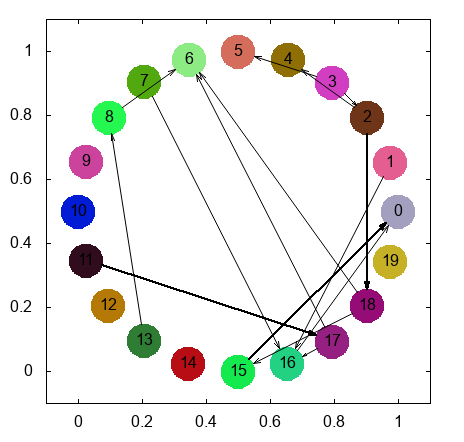
\includegraphics[width=0.7\textwidth]{grafoCircular}
    \centering
    \caption{Grafo con nodos dispuestos de manera circular, con algunos nodos unidos entre sí con arcos en color negro.}
    \label{grafoCircular}
  \end{figure}

  Un grafo en el que cada nodo puede estar solamente conectado a otros dos, de manera secuencial, es denominado árbol binario. A cada par de nodos conectados otro, se les denomina \textbf{hijos}, mientras que al nodo que se conectan se le llama \textbf{padre}. En ciertas aplicaciones computacionales, los árboles binarios son usados frecuentemente porque constituyen una manera eficiente de estructurar datos\cite{artComputerProgramming}. Mediante el paquete de desarrollo de grafos antes mencionado, se hizo un programa que genera árboles binarios dada una cantidad de ramas o capas. El código usado es el siguiente:

  \begin{lstlisting}[language=Python]
    from math import floor

    from Grafo import Grafo
    from Nodo import Nodo

    G = Grafo()

    niveles = 5
    hijos = 2
    maxNodosX = hijos ** niveles
    radioNodo = 1 / maxNodosX / 3
    yDesp = 1 / niveles

    nodo = Nodo()
    nodo.id = ""
    nodo.posicion = (0.5, 1)
    nodo.radio = radioNodo
    G.AgregarNodo(nodo)

    for nivel in range(1, niveles + 1):
        hijosNivel = hijos ** nivel
        xInicial = 1 / (hijosNivel * 2)
        for hijo in range(0, hijosNivel):
            n = Nodo()
            n.id = ""
            n.posicion = (xInicial + 1 / (hijosNivel) * hijo, 1 - yDesp * nivel)
            n.radio = radioNodo
            G.ConectarNodos(G.nodos[hijos ** (nivel - 1) - 1 + floor(hijo / hijos)], n)

        s = []
        s.append(nodo)
    G.Anchura(s, 0, True)
  \end{lstlisting}

  En este programa, se crean $2^n$ nodos por cada nivel del árbol, de un total de niveles definido en la línea $8$. En la línea $28$ se encuentra la función que conecta cada nodo con su padre correspondiente. El grafo resultante para 5 niveles se muestra en la figura \ref{arbolBinario} (p. \pageref{arbolBinario}).

  \begin{figure}[h]
    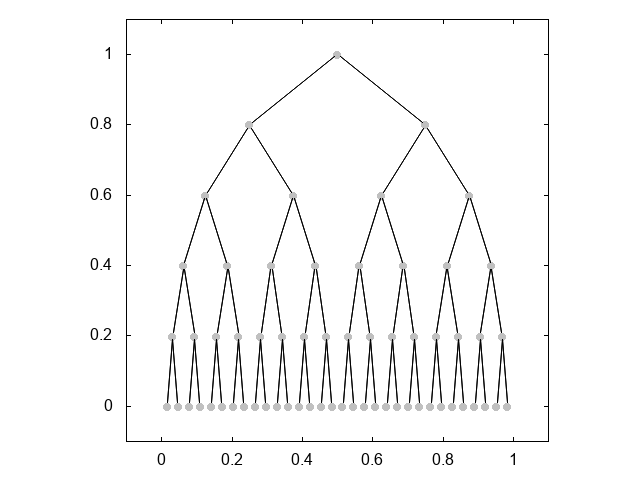
\includegraphics[width=0.7\textwidth]{arbolBinario}
    \centering
    \caption{Grafo del árbol binario de cinco niveles con que se probará el algoritmo de búsqueda en anchura.}
    \label{arbolBinario}
  \end{figure}

  El algoritmo de búsqueda en anchura consiste en recorrer, a partir de un nodo inicial denominado $s$, todos sus vecinos y luego, de cada vecino, recorrer sus vecinos y así recursivamente. Se llama \textbf{visitar} al hecho de que el algoritmo recorra determinado nodo. Una peculiaridad de este algoritmo, es que un nodo sólo puede ser visitado una sola vez. En este caso, se eligió como parámetro para marcar a un nodo visitado el uso de color rojo. Así, el algoritmo sólo visita nodos de un color distinto al rojo, por lo que inicialmente se colorearon de gris los nodos de este ejemplo. El algoritmo desarrollado genera una imagen \texttt{png} cada vez que el algoritmo visita a un nodo y, finalmente, las imágenes resultantes de cada visita fueron agrupadas en una animación \texttt{gif}. La animación puede verse en \url{https://github.com/jbenavidesv87/FlujoRedes/blob/master/ejemplos/06BFS/a.gif} y una secuencia de cuatro imágenes del algoritmo en la figura \ref{ejemploAnchura} (p. \pageref{ejemploAnchura}).

  \begin{figure}[h]
    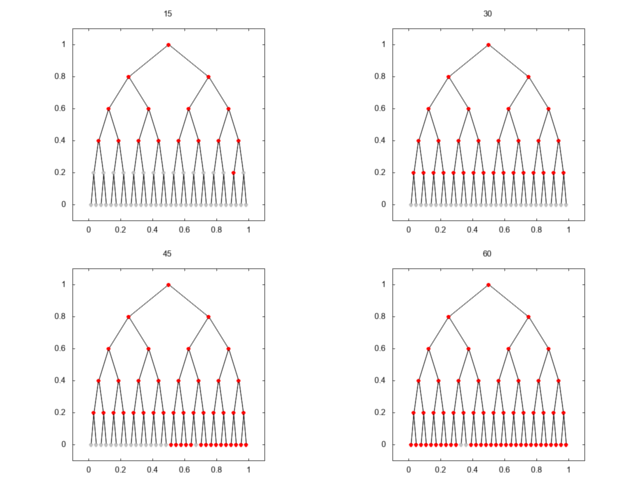
\includegraphics[width=0.7\textwidth]{ejemploAnchura}
    \centering
    \caption{Imágenes de las visitas $15$, $30$, $45$ y $60$ del grafo de ejemplo para este reporte.}
    \label{ejemploAnchura}
  \end{figure}

  El código del algoritmo, implementado en el paquete mencionado es el siguiente:

  \begin{lstlisting}[language=Python]
  def Anchura(self, s, i, debug = False):
    while len(s) > 0:
      n = s.pop()
      n.Color(255, 0, 0);
      if debug:
        self.nombre = "{:06d}".format(i)
        self.DibujarGrafo(titulo = str(i))
        remove('{:06d}.gnu'.format(i)) # https://pyformat.info/
      i = i + 1
      for v in self.vecinos[n]:
        if v.color != "#00ff0000":
          s.insert(0, v)
      if debug:
        self.Anchura(s, i, True)
      else:
        self.Anchura(s, i)
    return i
  \end{lstlisting}

  Este método, llamado \texttt{Anchura}, se incorporó dentro de la clase \texttt{Grafo} del paquete y recibe los siguientes parámetros:
  \begin{enumerate}
    \item \texttt{self}: El grafo sobre el que se ejecuta el método.
    \item \texttt{s}: Arreglo de nodos que contiene los siguientes nodos a ser recorridos.
    \item \texttt{i}: Una variable entera utilizada para contar el número de veces que se visita un nodo por primera vez.
    \item \texttt{debug}: Una variable booleana.
  \end{enumerate}

  En su primera iteración, se colorea el nodo \texttt{s} del que se parte (línea $3$); si la variable \texttt{debug} es verdadera, se genera una imagen \texttt{png} correspondiente al grafo resultante de esta iteración (líneas $4$ a $7$); se suma $1$ al iterador \texttt{i} (línea $8$); luego, por cada vecino del nodo \texttt{s}, si su color es distinto a rojo (línea $11$), se agrega este nodo a la lista de nodos por visitar y se repite esta iteración mientras haya nodos por visitar.

  El código completo descrito en este reporte, se halla en \url{https://github.com/jbenavidesv87/FlujoRedes/tree/master/ejemplos/06BFS}.

  \bibliography{biblio}
  \bibliographystyle{plain}

\end{document}
